\chapter{Near the Horizon}

These notes follow Leonard Susskind's seventh lecture on general relativity in the order in which the blackboard argument unfolds. We begin by stripping the Schwarzschild metric down to a dimensionless form, then use that simplification to estimate curvature, introduce proper distance from the horizon, and finally turn the geometry into causal questions about what Alice, Bob, and Charlie actually see. The present curation acknowledges Leonard Susskind, LazyingArt LLC, and Video2Book.

\section{Rescaled Schwarzschild Geometry}

The lecture opens in a practical mood. We go back to the Schwarzschild metric, not to admire it, but to clean it up. Susskind first writes the familiar formula with primed variables so that the primes can be discarded after rescaling. With \(r_{\mathrm S}=2MG\), we may write
\begin{equation}
d\tau^2
=
\left(1-\frac{2MG}{r'}\right)dt'^2
-
\frac{dr'^2}{1-\frac{2MG}{r'}}
-
r'^2\,d\Omega_2^2.
\end{equation}
He then defines
\begin{equation}
r=\frac{r'}{r_{\mathrm S}},
\qquad
t=\frac{t'}{r_{\mathrm S}},
\qquad
r_{\mathrm S}=2MG.
\end{equation}
Because we are using units with \(c=1\), time and length carry the same dimensions, so the same scale \(r_{\mathrm S}\) may be used for both. Substituting \(r'=r_{\mathrm S}r\) and \(t'=r_{\mathrm S}t\), we obtain
\begin{equation}
d\tau^2
=
r_{\mathrm S}^2
\left[
\left(1-\frac{1}{r}\right)dt^2
-
\frac{dr^2}{1-\frac{1}{r}}
-
r^2\,d\Omega_2^2
\right].
\end{equation}

\begin{remark}
A sign issue was caught from the room while the metric was being written on the board. We record only the corrected form. The lecture also writes the sphere metric in a convention-dependent way, but nothing in the present discussion depends on that detail, so \(d\Omega_2^2\) is the cleanest notation.
\end{remark}

This is the first payoff of the lecture. Every Schwarzschild black hole has the same dimensionless geometry. The only memory of the actual size of the hole is the overall factor \(r_{\mathrm S}^2\). That is why Susskind immediately says that, for most purposes, we may study the unit black hole with \(r_{\mathrm S}=1\). The analogy he gives is with spheres: all spheres have the same metric up to the square of their radius. So from this point on the lecture is really about the dimensionless metric inside the brackets.

\section{Curvature Scale at the Horizon}

Once the dimensional clutter is removed, the lecture pivots from notation to physics. Susskind does not launch into a full curvature computation. Instead he asks what the curvature near the horizon can possibly scale like.

The dimensional reasoning is the whole argument:
\begin{align}
[g_{\mu\nu}] &= 1,\\
[\Gamma] &\sim L^{-1},\\
[\mathcal R] &\sim L^{-2}.
\end{align}
The metric is dimensionless because it multiplies \(dx^\mu dx^\nu\), which already carries units of length squared. A Christoffel symbol contains one derivative with respect to position, and therefore scales as inverse length. The curvature tensor contains either a derivative of \(\Gamma\) or a product \(\Gamma^2\), so it must scale as inverse length squared.

Now we ask the question at the horizon, where \(r=1\). In the rescaled metric the only dimensionful quantity left is \(r_{\mathrm S}\). Therefore the curvature at the horizon must be of order
\begin{equation}
\mathcal R_{\text{horizon}} \sim \frac{1}{r_{\mathrm S}^2}.
\end{equation}
More generally, at any fixed dimensionless \(r\), the curvature must have the form
\begin{equation}
\mathcal R(r)\sim \frac{1}{r_{\mathrm S}^2}\,f_{\mathcal R}(r),
\end{equation}
for some dimensionless function \(f_{\mathcal R}(r)\).

This is where the lecture immediately converts mathematics into a physical statement. The larger the black hole, the larger \(r_{\mathrm S}\), and therefore the smaller the curvature at the horizon. Since tidal forces are curvature, a large black hole has milder tidal forces at the horizon than a small black hole. This is not a decorative observation. It is the permission slip for the later claim that crossing the horizon of a sufficiently large black hole need not be locally dramatic at all.

Susskind later makes that point vivid with examples. A solar-mass black hole, whose Schwarzschild radius is of order a kilometer, has violent tidal forces at the horizon. A supermassive black hole can have horizon tidal forces so weak that an ordinary person would notice nothing singular there.

\section{Proper Distance From The Horizon}

Once that physical point has been established, the lecture narrows deliberately. We set aside the angular factor for a while and concentrate on the radial-time geometry of the unit black hole. The next question is not ``what is the coordinate \(r\)?'' but ``what is the actual distance from the horizon?''

\begin{figure}[htbp]
\centering

\includegraphics[width=0.76\textwidth]{lecture_07_figure_02.png}
\caption{Blackboard sketch of the rescaled radial coordinate, with the horizon marked at \(r=1\).}
\end{figure}

\begin{figure}[htbp]
\centering
\begin{tikzpicture}[scale=1.1]
\draw[->] (0,0) -- (8,0) node[below] {$r$};
\fill (0,0) circle (1.2pt) node[below] {$0$};
\draw (2.4,0.14) -- (2.4,-0.14);
\draw (2.4,0.38) node[above] {horizon};
\draw (2.4,-0.34) node[below] {$1$};
\end{tikzpicture}
\caption{Clean redraw of the radial line used to define proper distance from the horizon.}
\end{figure}

The motivation matters. The lecture insists that \(r-1\) is not the proper distance from the horizon. It is only a coordinate difference. To obtain the actual radial distance, we compare two nearby points at the same time and with no change in angle. Thus
\begin{equation}
dt=0,
\qquad
d\Omega_2^2=0,
\end{equation}
and the metric reduces to
\begin{equation}
ds^2=\frac{dr^2}{1-\frac{1}{r}}.
\end{equation}
Therefore
\begin{equation}
ds=\frac{dr}{\sqrt{1-\frac{1}{r}}}.
\end{equation}
Now rewrite
\begin{equation}
1-\frac{1}{r}=\frac{r-1}{r},
\end{equation}
so that
\begin{equation}
ds=\sqrt{\frac{r}{r-1}}\,dr.
\end{equation}
This is the proper distance associated with a radial displacement \(dr\). The distance from the horizon to the point labelled by the coordinate \(r\) is therefore
\begin{equation}
\rho(r)=\int_1^r \sqrt{\frac{r'}{r'-1}}\,dr'.
\end{equation}

This is the mathematical hinge of the lecture. The lower limit is \(1\) because \(r=1\) is the horizon in the rescaled coordinates. The upper limit is the point whose distance from the horizon we want. Susskind remarks that the integral can indeed be done, but the closed form is not the point. The point is that \(\rho\) means proper distance from the horizon.

Now the whole reason for the change of variables becomes visible. Differentiate the definition:
\begin{equation}
\frac{d\rho}{dr}=\sqrt{\frac{r}{r-1}},
\qquad\text{hence}\qquad
d\rho^2=\frac{dr^2}{1-\frac{1}{r}}.
\end{equation}
So the ugly radial term in the metric has been engineered to become the simple term \(-d\rho^2\).

\section{The Metric In \(\rho\) And \(\omega\)}

The lecture now makes its next move. Since \(\rho\) has simplified the radial term, we keep it, and we also make one mild redefinition of time:
\begin{equation}
\omega=\frac{t}{2}.
\end{equation}
Susskind is explicit that this factor of \(2\) is merely convenient. It is not deep physics. He wants a time variable that makes the near-horizon metric take a suggestive form.

The blackboard shows the transformed metric very clearly on the right-hand side; the full equality is the standard completion consistent with the derivation we have just followed.

\begin{figure}[htbp]
\centering

\includegraphics[width=0.82\textwidth]{lecture_07_figure_03.png}
\caption{Blackboard form of the metric in \((\rho,\omega)\) variables, together with the far-field limit.}
\end{figure}

\begin{equation}
d\tau^2
=
F(\rho)\rho^2\,d\omega^2
-
d\rho^2
-
r(\rho)^2\,d\Omega_2^2.
\end{equation}
Here \(F(\rho)\) is defined implicitly. A student asks, in effect, whether \(F\) is simply being defined so that the time term looks like \(F(\rho)\rho^2 d\omega^2\), and Susskind answers yes. At this stage the split into \(F(\rho)\rho^2\) carries no content by itself. It is a convenience whose purpose will appear in the near-horizon limit.

The radial piece is now completely transparent:
\begin{equation}
-\frac{dr^2}{1-\frac1r}=-d\rho^2.
\end{equation}
That was the whole point of introducing \(\rho\).

The lecture now records just the information about \(F(\rho)\) and \(r(\rho)\) that will actually be needed. Far away from the hole,
\begin{equation}
\lim_{\rho\to\infty}F(\rho)\rho^2=4.
\end{equation}
This is simply the asymptotic statement that the time coefficient approaches its flat-space value once the definition \(\omega=t/2\) has been taken into account.

Near the horizon,
\begin{equation}
\lim_{\rho\to 0}F(\rho)=1,
\qquad
r(\rho)=1+\frac{\rho^2}{4}+\cdots.
\end{equation}
The second formula is only a near-horizon expansion, not an exact identity.

So near \(\rho=0\) the metric becomes
\begin{equation}
d\tau^2
\approx
\rho^2\,d\omega^2
-
d\rho^2
-
d\Omega_2^2.
\end{equation}
The lecture's real use of this is the radial-time part:
\begin{equation}
d\tau^2_{\text{radial-time}}
\approx
\rho^2\,d\omega^2-d\rho^2.
\end{equation}
This is the familiar flat Minkowski metric written in hyperbolic polar coordinates. If we recall the standard flat-space relations
\begin{equation}
X=\rho\cosh\omega,
\qquad
T=\rho\sinh\omega,
\end{equation}
then indeed
\begin{equation}
dT^2-dX^2=\rho^2\,d\omega^2-d\rho^2.
\end{equation}
So the lecture has arrived at the key geometric insight: near the horizon, the radial-time geometry looks like flat spacetime in unusual coordinates.

\section{Horizon, Interior, And Singularity}

Now the lecturer stops calculating and starts drawing. Once the metric has been rewritten in the right form, the rest of the argument is increasingly diagrammatic.

In hyperbolic polar coordinates, lines of constant \(\rho\) are hyperbolae and lines of constant \(\omega\) are rays. The limiting surface \(\omega=\infty\) lies along a null line. But \(\omega=\infty\) is just another way of saying the horizon. So the horizon is not merely a single point at the origin of the picture. It is the entire null line.

\begin{figure}[htbp]
\centering
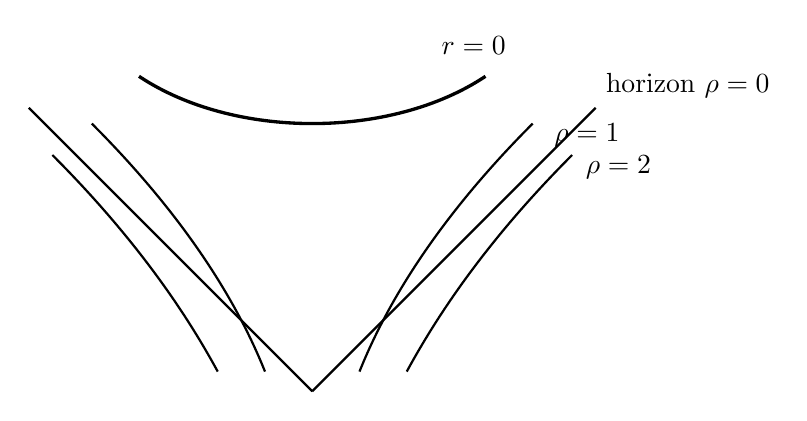
\begin{tikzpicture}[scale=1.0]
\draw[thick] (0,0) -- (3.6,3.6) node[above right] {horizon \(\rho=0\)};
\draw[thick] (0,0) -- (-3.6,3.6);
\draw[thick] (0.6,0.25) .. controls (0.9,1.0) and (1.5,2.1) .. (2.8,3.4);
\draw[thick] (1.2,0.25) .. controls (1.5,0.8) and (2.1,1.8) .. (3.3,3.0);
\draw[thick] (-0.6,0.25) .. controls (-0.9,1.0) and (-1.5,2.1) .. (-2.8,3.4);
\draw[thick] (-1.2,0.25) .. controls (-1.5,0.8) and (-2.1,1.8) .. (-3.3,3.0);
\draw[very thick] (-2.2,4.0) .. controls (-1.0,3.2) and (1.0,3.2) .. (2.2,4.0);
\draw (2.95,3.25) node[right] {\(\rho=1\)};
\draw (3.35,2.85) node[right] {\(\rho=2\)};
\draw (2.05,4.15) node[above] {\(r=0\)};
\end{tikzpicture}
\caption{Cautious reconstruction of the near-horizon causal picture. The horizon is the null line \(\rho=0\), and the singularity appears as the curve \(r=0\).}
\end{figure}

This is one of the lecture's deepest conceptual turns. In ordinary Euclidean geometry, making a radius small shrinks a circle toward a point. Here, making \(\rho\) small moves a hyperbola toward a null line. A tiny positive \(\rho\) does not pick out a tiny neighborhood of one point on the horizon. It picks out a whole hyperbola running close to the entire horizon. Thus the limit \(\rho\to 0\) reaches the whole null line, not just the tip.

Inside the horizon, the coordinate \(r\) becomes less than \(1\). In Susskind's language,
\begin{equation}
r>1 \Longleftrightarrow \rho^2>0,
\qquad
r<1 \Longleftrightarrow \rho^2<0.
\end{equation}
He is careful about the interpretation. This does not mean that space has literally turned into time or time into space as an invariant physical event. It means that the coordinates have a peculiar behavior across the horizon. The sign switch is a coordinate artifact.

What is not a coordinate artifact is the causal structure. Light rays remain \(45^\circ\) lines in the diagram. Once a timelike or null worldline lies beyond the horizon, every future-directed path is trapped inside the light cone, and every such path is driven toward smaller \(r\). Eventually one reaches
\begin{equation}
r=0.
\end{equation}
That is not a removable singularity. It is a genuine curvature singularity. The lecture stresses that curvature grows without bound there, and that no timelike or null observer inside the horizon can avoid it. In that sense the singularity is the true catastrophe; the horizon is the point of no return.

At this stage Susskind uses the name ``Kruskal coordinates.'' In the present lecture the important content is not the exact textbook coordinate transformation but the fact that the horizon has become a smooth null line and the singularity a separate, genuinely dangerous curve.

\section{Alice, Bob, Charlie, And The Rule: Draw The Diagram}

Once the geometry is in place, the lecture changes register. We no longer ask only what the metric looks like; we ask what different observers see. This is where the chapter must not flatten the discussion into a table. The rhythm of the lecture is question, diagram, and causal reading.

\begin{figure}[htbp]
\centering

\includegraphics[width=0.82\textwidth]{lecture_07_figure_04.png}
\caption{Blackboard sketch of Alice's infall, with the constant-time lines crowding against the limiting line \(t=\infty\).}
\end{figure}

\begin{figure}[htbp]
\centering
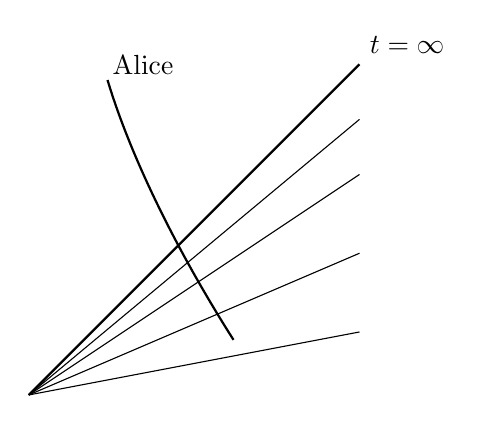
\begin{tikzpicture}[scale=1.0]
\draw[thick] (0,0) -- (4.2,4.2) node[above right] {\(t=\infty\)};
\draw[thin] (0,0) -- (4.2,0.8);
\draw[thin] (0,0) -- (4.2,1.8);
\draw[thin] (0,0) -- (4.2,2.8);
\draw[thin] (0,0) -- (4.2,3.5);
\draw[thick] (1.0,4.0) .. controls (1.3,3.0) and (1.9,1.8) .. (2.6,0.7);
\draw (1.45,3.95) node[above] {Alice};
\end{tikzpicture}
\caption{Simplified redraw of the causal sketch: constant Schwarzschild-time lines pile up against the horizon, while Alice's free-fall worldline passes through.}
\end{figure}

Here the board has acquired two different kinds of curves. The curved black families are constant \(r\) curves. The fanning straight lines are constant Schwarzschild-time curves, and the limiting one is labelled \(t=\infty\). With that in hand, the lecture starts posing puzzles.

\subsection{Question \& Answer}

\paragraph{Question.} Why does Alice cross the horizon in finite proper time if the horizon sits at \(t=\infty\)?

\paragraph{Answer.} Because \(t\) is not Alice's clock. In the exterior Schwarzschild description the horizon is the limiting surface \(t=\infty\), or more precisely \(\omega=\infty\). That is a statement about the coordinate slicing. Alice's own proper time is measured along her worldline, and in that time nothing singular happens at the crossing. The diagram shows the distinction immediately: the constant-\(t\) lines bunch up against the horizon, but Alice's trajectory goes straight through.

The lecture then sharpens the point. This is not merely a warning about bad coordinates. Bob, who remains outside at fixed distance from the hole, actually sees the same asymptotic approach. He receives light from Alice along \(45^\circ\) rays. Every later signal he receives comes from a point on Alice's worldline closer to the horizon. So if Bob stays outside forever, he sees Alice approach the horizon and never sees her cross it.

Susskind makes an even stronger claim. From Bob's point of view it is not just that he fails to witness the crossing. In Bob's own frame there is no sense in which Alice has already fallen through while he has somehow merely missed it. Everything Bob can observe, measure, or use operationally refers to Alice outside the horizon.

But Alice crosses nonetheless. Her proper time remains finite, her clock keeps ticking, and there is nothing special at the horizon itself. The only reason she cannot inform Bob afterward is that no signal from beyond the horizon can escape to him.

\subsection{Question \& Answer}

\paragraph{Question.} If Bob sees Alice slow down, does Alice see Bob speed up?

\paragraph{Answer.} No. This is the next trap the lecture wants us to avoid. Bob sees Alice slow down because the later and later light rays arriving from her come from events ever closer to the horizon. Her clocks appear to him to run more and more slowly. But Alice does not see some reciprocal runaway on Bob's side.

She sees Bob in her past, to be sure, but everyone sees everyone else in the past; all observation runs along light cones. That is not yet a special black-hole effect. What matters is the causal asymmetry. Bob, remaining outside, eventually loses the ability to receive signals from Alice. Alice, after crossing, can still look back and see Bob for a while. What terminates her observations is not a dramatic change in Bob. It is the end of her own worldline at the singularity.

The lecture presses this point with a vivid operational statement. If Bob stays outside forever, then in his own time he sees Alice for an infinite duration, but he sees only a finite number of heartbeats. In that restricted and slightly foolish sense he may say that he sees Alice die at the horizon. But this is a statement about the observational record of an accelerated outside observer. It is not a local event on Alice's worldline. She remains perfectly ordinary until she gets near the singularity.

There is one more nuance in the lecture. If Bob does not hover forever, but instead eventually falls in late enough, then he can see a little bit of Alice after she has crossed the horizon. But he does not gain much. Having crossed late, he is very quickly terminated by the singularity. So even this refinement preserves the same lesson: the asymmetry comes from the causal structure, not from a naive mirror symmetry between Bob's and Alice's clocks.

\subsection{Question \& Answer}

\paragraph{Question.} What does Charlie see if he follows Alice in free fall?

\paragraph{Answer.} Charlie sees nothing special at the horizon. This is the cleanest operational test of the claim, established earlier by the curvature estimate, that the horizon of a sufficiently large black hole is locally mild. If Charlie falls just behind Alice, both of them are in free fall. They can exchange light signals, talk to each other, even hold hands. Near the horizon their motion is, to an excellent approximation, the motion of ordinary inertial observers in nearly flat spacetime.

The lecture is explicit: Charlie sees Alice as a perfectly normal infalling companion. If he knows where the horizon is by prior calculation, he will see her cross it at the same stage of his own fall at which he reaches it. There is no signpost there. Nothing sudden happens. And after he crosses, he can look back and see that she is inside.

The same goes the other way. Alice sees Charlie as another ordinary free-falling observer. The two of them can converse back and forth. The dramatic asymmetry of the Bob story is absent because Charlie is not holding himself up outside the hole. He is not an accelerated outside observer. He is sharing the infall.

The lecture adds one more useful refinement. If Charlie changes his mind at the last moment and accelerates hard enough to stay outside, then he joins Bob's class of observers and no longer sees Alice cross the horizon. So the real contrast is not ``Charlie versus Bob'' as personalities. It is free fall versus accelerated hovering.

\begin{figure}[htbp]
\centering

\includegraphics[width=0.82\textwidth]{lecture_07_figure_05.png}
\caption{Causal answer diagram for the observer questions.}
\end{figure}

\begin{figure}[htbp]
\centering
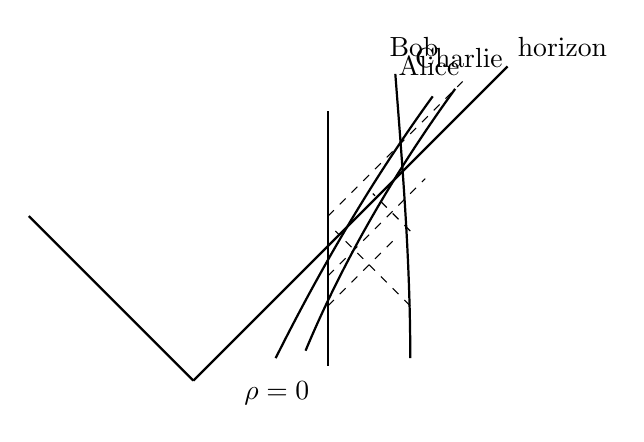
\begin{tikzpicture}[scale=0.95]
\draw[thick] (0,0) -- (4.2,4.2) node[above right] {horizon};
\draw[thick] (0,0) -- (-2.2,2.2);
\draw[thick] (1.8,0.2) -- (1.8,3.6);
\draw[thick] (2.9,0.3) .. controls (2.9,1.6) and (2.8,2.8) .. (2.7,4.1);
\draw (2.95,4.2) node[above] {Bob};
\draw[thick] (1.1,0.3) .. controls (1.7,1.5) and (2.4,2.7) .. (3.2,3.8);
\draw (3.15,3.95) node[above] {Alice};
\draw[thick] (1.5,0.4) .. controls (2.0,1.6) and (2.7,2.8) .. (3.5,3.9);
\draw (3.55,4.05) node[above] {Charlie};
\draw[dashed] (1.8,1.0) -- (2.7,1.9);
\draw[dashed] (1.8,1.4) -- (3.1,2.7);
\draw[dashed] (1.8,1.8) -- (3.4,3.4);
\draw[dashed] (1.8,2.2) -- (3.6,4.0);
\draw[dashed] (2.9,1.0) -- (1.9,2.0);
\draw[dashed] (2.9,2.0) -- (2.4,2.5);
\draw (0.55,0.12) node[below right] {\(\rho=0\)};
\end{tikzpicture}
\caption{Simplified causal construction. The answer comes from drawing worldlines and null rays, not from verbal symmetry arguments alone.}
\end{figure}

By the end of the lecture the method itself has become explicit. If one wants to know who sees what, the right procedure is not to speculate verbally. One draws the diagram, draws the light rays, and reads the answer off from causality. Susskind says it bluntly: the diagram is all you really need.

\section{What The Diagram Does And Does Not Yet Answer}

The lecture is equally careful about scope. The diagram is powerful, but it is not yet the whole story of realistic black-hole physics.

First, only part of the idealized diagram is physically relevant for a black hole formed by collapse. Susskind says this repeatedly near the end. The upper-right region is the one of present interest. The lower half and the apex of the eternal extension are not to be read as literal features of an astrophysical collapse. So even though the mathematical diagram can be drawn in full, only a portion of it corresponds to the physical black holes we expect to form in nature.

Second, if appreciable matter falls in, the mass of the black hole changes, and therefore so does \(r_{\mathrm S}\). The lecture explicitly postpones the detailed discussion of how the horizon forms and how it grows. We are told only the rough qualitative picture: if a sufficiently heavy object falls in, the horizon bulges outward, merges, and then settles down into a slightly larger sphere. That is the business of the next lecture.

Third, the light we see from astrophysical black holes does not come from the horizon itself. It comes from outside the horizon: accretion disks, hot matter, orbiting photons, collisions, and all the complicated business of real environments. The present lecture is really about an idealized Schwarzschild black hole in otherwise empty space.

Fourth, rotation changes the geometry. The lecture touches this only in passing, but enough to mark the boundary. Rotating holes are not described by the simple spherically symmetric picture used here; the horizon is deformed, the geometry changes, and the singularity structure is different.

Fifth, the late historical remarks belong in the margin of the chapter rather than in its central derivation, but they do matter as orientation. The names Finkelstein, Eddington, Kruskal, and Wheeler appear because the lecture wants to remind us that the smoothness of the horizon was not obvious from the original Schwarzschild form, and that the slogan ``black holes have no hair'' is part of the later understanding of how horizons settle down.

Finally, the lecture comes back to the scaling that opened the whole discussion. Once we scale out \(r_{\mathrm S}\), the dimensionless causal diagram does not change shape when \(r_{\mathrm S}\) changes. What changes is the meaning of lengths and times measured on it. The number of meter sticks between two points, or the amount of proper time represented by a segment, scales with \(r_{\mathrm S}\). Thus the same dimensionless picture can describe both a one-kilometer black hole and a monster of \(10^9\) solar masses, even though the physical sizes involved are utterly different.

\section{Summary}

The lecture has a clean spine. We rescale the Schwarzschild metric so that every black hole shares the same dimensionless geometry up to the overall factor \(r_{\mathrm S}^2\). We then use dimensional analysis to see that curvature at the horizon is of order \(1/r_{\mathrm S}^2\), which explains why large black holes have weak horizon tidal forces. Next we replace the coordinate \(r\) by the proper-distance variable \(\rho\), define \(\omega=t/2\), and rewrite the near-horizon metric so that its radial-time sector becomes flat spacetime in hyperbolic polar coordinates.

From there the lecture turns geometry into causality. The horizon is not a point but a null line. The interior is the region \(r<1\), and every future-directed timelike or null trajectory inside it hits the true singularity at \(r=0\) in finite proper time. Bob, remaining outside, never sees Alice cross the horizon. Alice experiences nothing special at the crossing. Charlie, if he follows her in free fall, also sees nothing special there. The methodological moral is the one Susskind insists on at the blackboard: if one wants to know who sees what, one should draw the diagram and follow the light rays.